\chapter{Experimental Methods}
In this chapter I will describe the experiments I conducted for this thesis. The first section will deal cover the configuration and customization of the continuous wave (CW) Titanium Sapphire laser I used as an excitation source for conducting both PLE and $\mu$PL experiments. Section two will cover the design and construction of the in-cryostat optic mount for the $\mu$PL experiment as well as the optical configuration for data collection. Section three will illustrate the data collection procedure used in $\mu$PL experiments, as well as the function and implementation of LabView code I wrote for hardware control and data acquisition. In section four, I will lay out the optical design of our PLE experiments and in section five, I will discuss the experimental data collection process and signal optimization routines.

\section{The Light Source}
\indent The PLE and $\mu$PL experiments required a CW laser light source with a few properties: the laser must be a stable and fairly high-power light source with narrow line-width. For $\mu$PL, it was important that we have a fairly Gaussian and symmetric beam so we could obtain the desired spot-size and resolution at the sample. Additionally, conducting PLE scans required that we have the ability to computer control the laser wavelength over a fairly broad range of wavelengths, roughly a spectral region from $\lambda = 780$nm to $\lambda = 850$nm. The laser we chose for this task was a Schwartz Electro Optics Titan-CW Titanium Sapphire (Ti:Sapph) laser. Its specifications were fairly close to our needs, as its specified operating power is 500mW with a tunable range from roughly 700-820nm CITE Titan manual. 

\indent The laser cavity can be configured for either CW or pulsed operation. In CW operation a 532nm pump beam, 5W of power, enters the cavity through a series of steering mirrors. After entering, the pump passes through a lens to focus the pump on the Ti:Sapph crystal. After the gain medium, the remaining pump light passes through the end mirror and terminates at the back of the laser enclosure. The laser configuration is shown in figure 3.1.
\begin{figure}[h!]
\centering
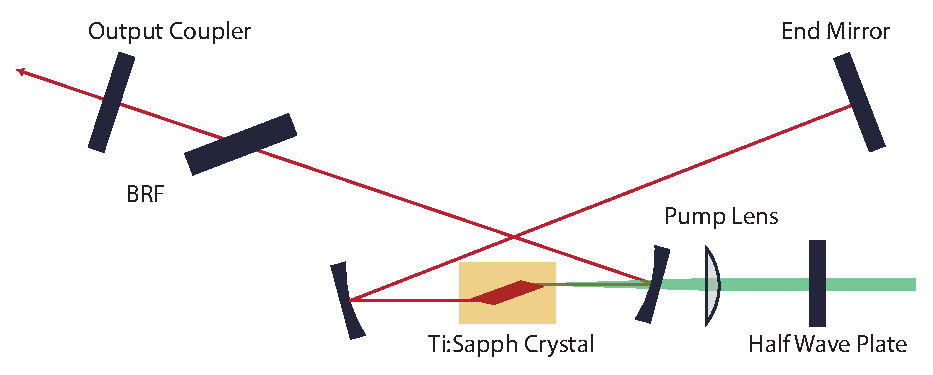
\includegraphics[width = .8\textwidth]{laser.eps}
\caption{ \doublespacing A depiction of the modified mount: the actuator arm fits into a sleeve attached by a pivot to the rotating filter mount. A spring attached to both the rotating mount and aluminum block holds the sleeve to the actuator and ensures smooth rotation in either direction.}
\label{lasercav}
\end{figure}

\indent Though the Ti:Sapph laser nearly met our specifications, it required two modifications to be operable in our experiments. First, we needed to add a computer controlled actuator to rotate the the birefringent tuner in order to allow for increased tenability and repeatability relative to a manually actuated micrometer. We modified the rotation mount for the birefringent filter (BRF) to accommodate a Newport TRB25 linear actuator. The linear actuator pushed a spring-loaded arm to rotate the BRF to a specified angle and select our desired wavelength. Figure \ref{brfmount} depicts the modified BRF mount with the actuator attached.
\begin{figure}[h!]
\centering
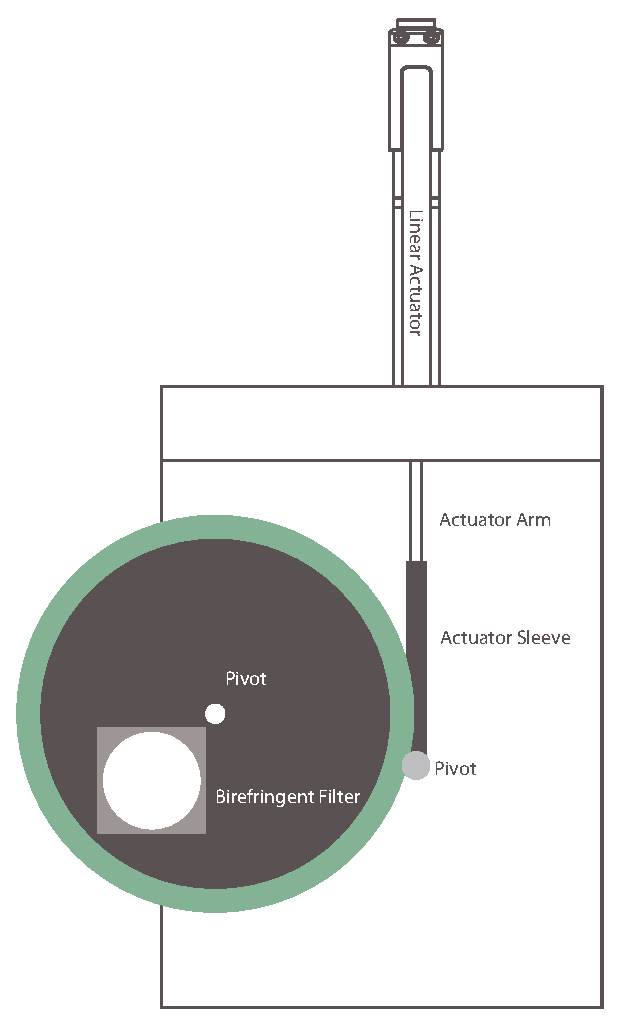
\includegraphics[width = .35\textwidth]{Actuator.eps}
\caption{ \doublespacing A depiction of the modified mount: the actuator arm fits into a sleeve attached by a pivot to the rotating filter mount. A spring attached to both the rotating mount and aluminum block holds the sleeve to the actuator and ensures smooth rotation in either direction.}
\label{brfmount}
\end{figure}

\section{Optical Components and Optical Path Configuration for Microphotoluminescence Experiments}

\subsection{Manufacturing the SIL}

\indent In order to obtain the resolution necessary to image disorder, the experiment employed a solid immersion lens (SIL) at the surface of the sample to increase the index of refraction at the imaging plane. I chose ZnSe as the SIL material, as its index of refraction at 780nm is n=2.53 CITE website. However, ZnSe SILs are not commercially available, so I resorted to manufacturing SILs from a stock ZnSe window. The window measured 2.54cm diameter by 1cm thickness, and our goal was to manufacture SILs of roughly 3mm in radius. To begin, we used a core drill, diameter 6.35mm, to cut out a cylindrical chunk of ZnSe. I then centered and glued the cylindrical stock material to a brass dowel, 2mm in radius. After the ZnSe was glued to the rod, the SIL shaping began. I put the brass dowel in a power drill used 200 grit sandpaper to shape the ZnSe cylinder roughly into a hemisphere.

\indent  When the SIL was in the roughly correct shape, we lapped and polished the hemispherical surface until the SIL was at the correct size. Additionally, since the experiment required optical quality surfaces, this was a careful and fairly lengthy process. I made the polishing lapps by machining a 2.54cm diameter copper rod to roughly 2cm in diameter with a 1.8cm wide by 1cm deep cavity. Then, I melted lead solder into the cavity, let it harden, and machined the face of the copper and solder until they were flush and mahcine-smooth. Then, I pressed a cleaned, 6.35mm dieameter ball bearing halfway into the solder. Figure 3.3 depicts what a finished lapp looked like before it was used to grind and polish the SIL. 

\begin{figure}[h!]
\centering

\includegraphics[width = .3\textwidth]{lapp.eps}
\caption{ \doublespacing A depiction of the lapp. The orange casing is copper while the grey lining is lead solder. The cavity left by the ball bearing was smooth enough to polish the relatively soft ZnSe hemispheres.}
\label{lapp}
\end{figure}



\indent After the lapp was made, we mounted the dowel with the SIL still attached to a glass lathe. As the lathe rotated, we placed the lapp with a mixture of glass polishing solution of various grit and mineral oil onto the SIL and held it in place with a sharpened wire. The wire and Lapp were both off center so the friction of the rotating SIL would randomly move the lapp so as to evenly polish the surface of the hemisphere. A depiction of this setup is in figure \ref{polish}. (GRIT SIZE INFO). After the polishing process finished, the SIL was removed from the dowel and the flat surface was poilshed with a colloidal silicon mixture. When the SIL was finished, we had a hemispherical (to within 1\%) ZnSe SIL.

\begin{figure}[h!]
\centering

\includegraphics[width = .8\textwidth]{lathe.eps}
\caption{ \doublespacing A depiction of the polishing setup in the lathe. The off-center placement of the lapp and lapp pin allowed the lapp to rotate and move slightly to randomize the SIL polishing.}
\label{polish}
\end{figure}

\subsection{Manufacturing the Cryostat Optics Mount}
\indent In order to achieve the desired imaging resolution, our chosen optical geometry (refer to \ref{confocal2}) required a high-NA lens as the imaging lens. We therefore chose an Edmund Optics $0.83NA$, 9mm effective focal length aspheric lens. Together with our ZnSe SIL, this gave us an Abbe diffraction limit of $d = 185.05$nm for PL centered around $\lambda = 780$nm. This diffraction limit is less than our goal of $d = 200$nm. As our experiment required cooling to cryogenic temperatures, we had to build a mechanically and thermally stable optics platform to hold the lenses and QW sample together in the correct configuration. Therefore, working with our machinists, I designed the optics mount int \ref{mount}. The optics mount stands vertically in our Cryo-Con 8CN bath cryostat. Therefore, since the excitation laser enters the cryostat vertically, we designed the optics mount to be held to a mirror which filled the entire optics mount and was positioned at $45\deg$ so as to direct the laser to the sample and capture the total PL image. The mirror was ground by taking a stock Thor Labs 2.54cm diameter mirror, protecting the silvered face with weak glass tape, cutting the mirror to 3mm thick, and securing the mirror to an aluminum rod of 15mm diameter (the same diameter as the inside of the optic mount). The end of the rod was bevelled at a $45\deg$ angle, and the mirror and rod combination was spun by hand on the side of a glass cutting sawblade. This process ensured that, when the glass was cut flush with the edge of the rod, the mirror was the correct elliptical shape and diameter to fit in the optics mount. The mirror was then secured to a roughly .5mm thick sheet of indium which was epoxied to the mirror mount. 

\subsection{Experimental Optical Path Configuration}
\indent Our aim was to characterize disorder over an area roughly $200\mu$m in diameter. In order to do so, we needed the laser spotsize to be $200\mu$m in diameter or larger. Additionally, to obtain clear images, the excitation spot needed to be monotonic, symmetric, and preferably Gaussian in shape. To this end, I characterized the laser spot size and found it to be $1.6\pm.1$mm FWHM diameter, roughly Gaussian and symmetric to within 20\%. In order to obtain the requisite beam diameter at the sample, it was necessary to resize the beam going into the cryostat. In order to do so, we used four lenses to resize the beam. The first two lenses, one of focal length 60mm and the other of focal length 25.4mm, shrunk our beam from 1.6mm to 0.68mm. The second lens in the second pair of lenses was the in-cryostat asphere, and in combination with the lens outside the cryostat, focal length 30mm, resized our beam to $203\mu$m in diameter. After the beam hit the sample, the PL signal travelled through the asphere and out of the cryostat. We placed a 90\% reflective non-polarizing beamsplitter (NPBS) outside the cryostat to pick off the PL signal. The beamsplitter sent the PL signal through an achromatic, 20cm focal length lens, and a a polarizer to filter out the laser. Finally, the signal focused onto the slit of a Horiba iHR550 imaging spectrometer. The 20cm lens was 50.4cm in diameter and mounted to a linear translation stage. Its function was to focus the PL spot on the spectrometer slit and translate the image across the spectrometer slit, as in Figure \ref{slit}. The PL image was roughly 9mm in radius at the lens, so since the lens is relatively large, spherical image aberrations during image translation were negligible.

\begin{figure}[h!]
\centering
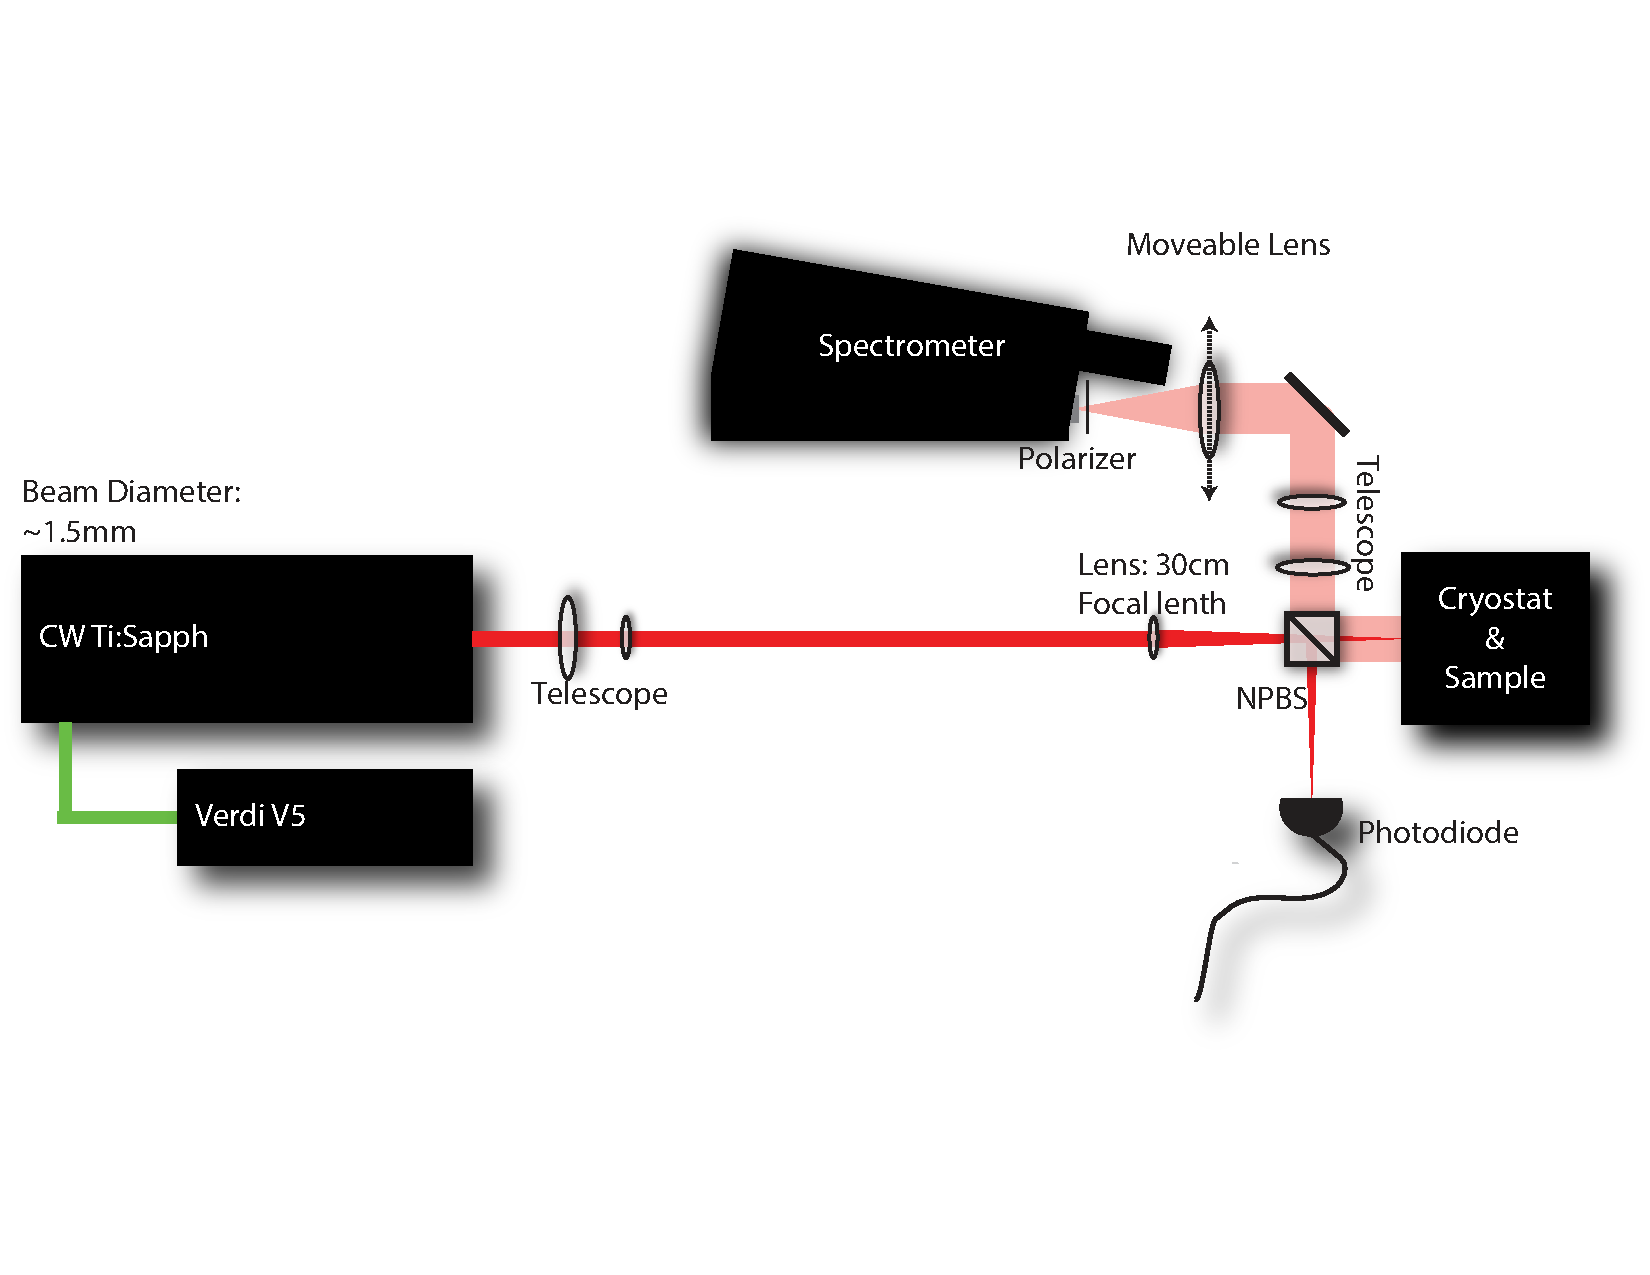
\includegraphics[width = \textwidth]{upl.pdf}
\caption{ \doublespacing A diagram of the experimental components. The second telescope was an optional feature, its use doubled the system magnification.}
\label{upl}
\end{figure}
\begin{figure}[h!]
\includegraphics[width = .5\textwidth]{specslit.eps}
\caption{ \doublespacing A depiction of the PL spot on the spectrometer slit. The spot translates across the slit as we move the lens on the translation stage, allowing us to take vertical slices of the image as it translates across the slit.}
\label{slit}
\end{figure}
\indent We monitored the laser power with a photodiode, using the light that was dumped out of the experiment by the NPBS. Additionally, between the NPBS and the moveable lens, we had the option to add a telescope to improve the magnification of the system further. The use of the telescope depended on the intensity of the signal. If the signal was vanishingly small, the telescope made it nearly unreadable. Therefore, in cases where less signal reached the spectrometer, the telescope became impractical.

\section{Microphotoluminescence Data Collection}
\subsection{Optical Alignment Considerations}
When the optical components were roughly in the configuration seen in Figure \ref{upl}, we cooled the sample to $10\pm1$k and adjusted the laser power to 100mW so that the laser power at the sample was 1mW (because the NPBS dumped 90\% of the power we fed into it. We identified the PL signal using a polarization filter, as it was the only signal left after the filter was rotated such that its polarization was orthogonal to that of the beam. Then, we experimentally adjusted the focus of the moveable



